\documentclass{standalone}

\usepackage{tikz}

\usetikzlibrary{patterns}
\usetikzlibrary{arrows.meta}

\usepackage{bm}

\begin{document}

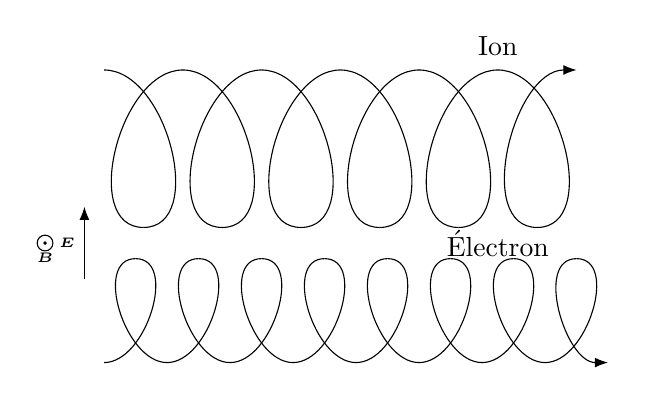
\begin{tikzpicture}

	\def\offsetion{0.5}
	\def\widthion{2*\offsetion}
	\def\heightion{-2}
	
	\def\offsete{0.4}
	\def\widthe{2*\offsete}
	\def\heighte{-0.66*\heightion}

	\def\nion{4}
	\def\ne{6}

	\foreach \i in {0, ..., \nion} {
		\draw (\i*\widthion, 0) to[ out=0, in=0 ] (\i*\widthion+\offsetion, \heightion);
		\draw (\i*\widthion+\offsetion, \heightion) to[ out=180, in=180 ] (\i*\widthion+\widthion, 0);	
	}
	\draw (\nion*\widthion+\widthion, 0) to[ out=0, in=0 ] (\nion*\widthion+\widthion+\offsetion, \heightion);
	\draw[ -{Latex} ] (\nion*\widthion+\widthion+\offsetion, \heightion) to[ out=180, in=180 ] (\nion*\widthion+\widthion+\widthion, 0);	
	
	\node[ align=right ] at (\nion*\widthion+\widthion, 0.3) {Ion};
	
	\foreach \i in {0, ..., \ne} {
		\draw (\i*\widthe, \heightion-\heighte*1.3) to[ out=0, in=0 ] (\i*\widthe+\offsete, \heightion-\heighte*0.3);
		\draw (\i*\widthe+\offsete, \heightion-\heighte*0.3) to[ out=180, in=180 ] (\i*\widthe+\widthe, \heightion-\heighte*1.3);	
	}
	\draw (\ne*\widthe+\widthe, \heightion-\heighte*1.3) to[ out=0, in=0 ] (\ne*\widthe+\widthe+\offsete, \heightion-\heighte*0.3);
	\draw[ -{Latex} ] (\ne*\widthe+\widthe+\offsete, \heightion-\heighte*0.3) to[ out=180, in=180 ] (\ne*\widthe+\widthe+\widthe, \heightion-\heighte*1.3);	
	
	\node[align=right] at (\nion*\widthion+\widthion, \heightion-\heighte*0.15) {Électron};
	
	\draw[ -{Latex} ] (-0.25, \heightion-\heighte*0.5) -- (-0.25, \heightion+\heighte*0.2) node[midway, anchor=east] {\tiny \( \bm{E} \)};
	
	\fill (-0.75, \heightion-\heighte*0.15) circle [radius=0.025];
	\draw (-0.75, \heightion-\heighte*0.15) circle [radius=0.1] node[ anchor=north ] {\tiny \( \bm{B} \)};

\end{tikzpicture}

\end{document}